\chapter{Governing Equations} \label{chap:governing-equations}
\section{Governing Equations for Flow in Magnetic Nozzle}
In this section, we will derive the governing equations of the flow in magnetic nozzle, starting from the fluid description for plasma.

In magnetic nozzle, the magnetic field is along the nozzle, which we denote as z-axis. Due to Lorentz force, the charged particles gyrates about the magnetic field lines. Because the magnetic moment is invariant in such situation (\textbf{reference}). The fluid velocity of particles can be written as $\mathbf{v} = v\mathbf{B}/B$, meaning that the particles move along the magnetic field lines. Therefore the conservation of density 
\[ 
\pdv{n}{t} + \div(n\mathbf{v}) = 0 
\Rightarrow 
\pdv{n}{t} + B\pdv{z}(\frac{nv}{B}) = 0  
\]
In the derivation, $\div{\mathbf{B}} = 0$ is used.

To derive the second governing equation, we start from the conservation of momentum, 
\[ \pdv{v}{t} + v\pdv{v}{z} = -\frac{1}{\rho}\grad{p} \]
Let $\grad{p} = k_BT\pdv*{n}{z}$, we have
\[ \pdv{v}{t} + v\pdv{v}{z} = -c_s^2\frac{1}{n}\pdv{n}{z} \]
where $c_s^2 = k_BT/m$ is the square of sound speed.

Therefore the dynamics of the flow in magnetic nozzle can be characterized by the conservation of density and momentum,
\begin{align*}
	&\pdv{n}{t} + B\pdv{z}(\frac{nv}{B}) = 0\\
	&\pdv{v}{t} + v\pdv{v}{z} = -c_s^2\frac{1}{n}\pdv{n}{z}
\end{align*}
The discussion of magnetic field is in next subsection.


\subsection{Magnetic Field in Magnetic Nozzle}
In 1D problem, the magnetic field is given by
\[ B(z) = B_0 \left[1 + R\exp(-\left(\frac{x}{\delta}\right)^2)\right] \]
where $1+R$ is the magnetic mirror ratio, and $\delta$ determines the spread of the magnetic field. It is shown in Fig.(\ref{fig:magnetic-field}).
\begin{figure}[H]
	\centering
	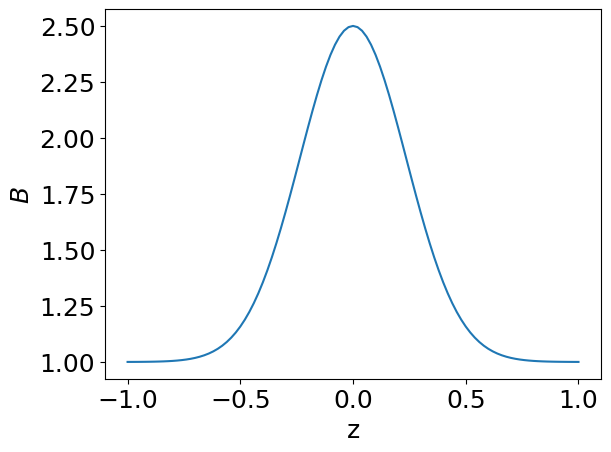
\includegraphics[width=0.7\linewidth]{img/governing-equations/magnetic-field}
	\caption{This is the magnetic field in nozzle with mirror ratio $1+R=B_{max}/B_{min}=2.5$, and the spread of magnetic field, $\delta=0.1/0.3=0.\bar{3}$. }
	\label{fig:magnetic-field}
\end{figure}


\subsection{Velocity Profile at Equilibrium}
Let $n_0$ and $v_0$ be the density and velocity at equilibrium (stationary solution), we know that $\pdv*{n_0}{t}=0$ and $\pdv*{v_0}{t}=0$, therefore $n_0$ and $v_0$ satisfy the so-called equilibrium condition,
\begin{align*}
	&\pdv{z}(\frac{n_0v_0}{B}) = 0 \\
	&v_0\pdv{v_0}{z} = -c_s^2\frac{1}{n_0}\pdv{n_0}{z} 
\end{align*}

Let $M(z) = v_0(z)/c_s$ be the mach number (nondimensionalized velocity). The equations of motion become
\begin{align*}
	&B\pdv{z}(\frac{n_0M}{B}) = 0\\
	&M\pdv{M}{z} = -\frac{1}{n_0}\pdv{n_0}{z}
\end{align*}
Substitute $\frac{1}{n_0}\pdv*{n_0}{z}$ using first equation, the conservation of momentum becomes
\[ (M^2-1)\pdv{M}{z} = -\frac{M}{B}\pdv{B}{z} \]

Notice that there is a singularity at $M=1$, the sonic speed.

This is a separable equation, integrate it and use the conditions at midpoint $B(0)=B_m, M(0)=M_m$ we get
\[ M^2e^{-M^2} = \frac{B^2}{B_m^2}M_m^2e^{-M_m^2} \]
We can now express $M$ using the Lambert W function,
\[ M(z) = \left[ -W_k\left(-\frac{B(z)^2}{B_m^2}M_m^2e^{-M_m^2}\right) \right]^{1/2} \]
where the subscript $k$ of $W$ stands for branch of Lambert W function. When $k=0$, it is the subsonic branch; When $k=-1$, it is the supersonic branch. Below shows a few cases of the solution.
\begin{itemize}
	\item $M_m < 1, k=0$, subsonic velocity profile.
	\item $M_m = 1$, $k=0$ for $x<0$ and $k=-1$ for $x>0$, accelerating profile
	\item $M_m = 1$, $k=-1$ for $x<0$ and $k=0$ for $x>0$, decelerating profile
	\item $M_m > 1, k=-1$, supersonic velocity profile
\end{itemize}
 Fig.(\ref{fig:velocity-profiles}) shows some cases of the solution.
\begin{figure}[H]
	\centering
	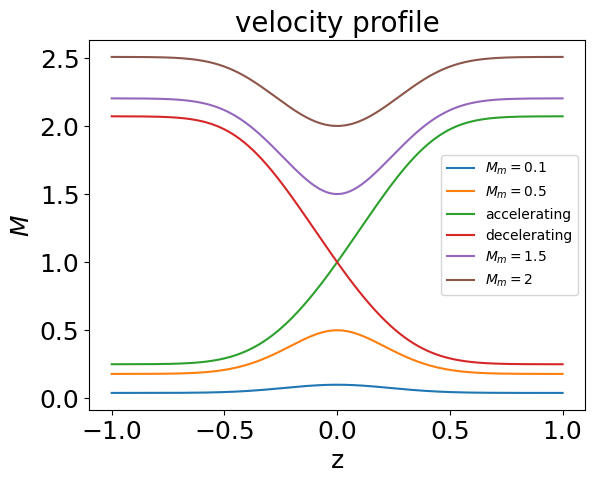
\includegraphics[width=0.7\linewidth]{img/governing-equations/velocity-profiles}
	\caption{The velocity profile in the magnetic nozzle is completely determined by $M_m$, the velocity at the midpoint, $z=0$. For the transonic velocity profiles, $M_m$ alone is not enough to determine the profile, we need to specify the branch of Lambert W function to determine whether it is accelerating or decelerating.}
	\label{fig:velocity-profiles}
\end{figure}



\section{Linearized Equations}
For convenience, we nondimensionalize the governing equations by normalizing the velocity to $c_s$, $v\mapsto v/c_s$, $z$ to system length $L$, $z \mapsto z/L$ and time $t\mapsto c_s t/L$. The governing equations become
\begin{align}
    &\pdv{n}{t} + n\pdv{v}{z} + v\pdv{n}{z} - nv\frac{\partial_z B}{B} = 0 \\
    &n\pdv{v}{t} + nv\pdv{v}{z} = -\pdv{n}{z}
\end{align}
and the nondimensionalized equilibrium condition is
\begin{align}
    &\pdv{z}(\frac{n_0v_0}{B}) = 0 \label{eq:equilibrium-convervation-of-mass}\\
    &v_0\pdv{v_0}{z} = -\frac{1}{n_0}\pdv{n_0}{z} \label{eq:equilibrium-convervation-of-momentum}
\end{align}

Now we are going to derive an important intermediate result, the linearized governing equations.
\begin{proposition}
    Let $n = n_0(z) + \tilde{n}(z,t)$ and $v = v_0(z) + \tilde{v}(z,t)$, where $\tilde{n}$ and $\tilde{v}$ are small perturbed quantities. The linearized governing equations are
    \begin{align}
        &\frac{1}{n_0}\pdv{\tilde{n}}{t} 
        + \pdv{\tilde{v}}{z} + v_0\tilde{Y} + \tilde{v}\frac{\partial_z n_0}{n_0} - \tilde{v}\frac{\partial_z B}{B} = 0 
        \label{eq:linearized-conservation-of-mass}
        \\
        &\pdv{\tilde{v}}{t} + \pdv{(v_0\tilde{v})}{z} = -\tilde{Y}
        \label{eq:linearized-conservation-of-momentum}
    \end{align}
    where 
    \[ \tilde{Y} \equiv \frac{1}{n_0}\pdv{\tilde{n}}{z} - \frac{\partial_z n_0}{n_0^2}\tilde{n} = \pdv{z}(\frac{\tilde{n}}{n_0}) \]
\end{proposition}
\begin{proof}
    We first derive Eq.(\ref{eq:linearized-conservation-of-mass}). We linearize Eq.(\ref{eq:equilibrium-convervation-of-mass}) by setting $n=n_0+\tilde{n}$ and $v=v_0+\tilde{v}$. By ignoring the second order perturbations, we obtain
    \begin{align*}
        &\pdv{(n_0+\tilde{n})}{t} 
        + (n_0+\tilde{n})\pdv{(v_0+\tilde{v})}{z} 
        + (v_0+\tilde{v})\pdv{(n_0+\tilde{n})}{z} 
        - (n_0+\tilde{n})(v_0+\tilde{v})\frac{\partial_z B}{B} = 0 \\
        \Rightarrow 
        &\pdv{\tilde{n}}{t} 
        + n_0\pdv{v_0}{z} + \tilde{n}\pdv{v_0}{z} + n_0\pdv{\tilde{v}}{z}
        + v_0\pdv{n_0}{z} + \tilde{v}\pdv{n_0}{z} + v_0\pdv{\tilde{n}}{z} 
        - (n_0v_0 + n_0\tilde{v} + \tilde{n}v_0)\frac{\partial_z B}{B} = 0 \\
        \Rightarrow
        &\frac{1}{n_0}\pdv{\tilde{n}}{t} 
        + \pdv{v_0}{z} + \frac{\tilde{n}}{n_0}\pdv{v_0}{z} + \pdv{\tilde{v}}{z}
        + \frac{v_0}{n_0}\pdv{n_0}{z} + \frac{\tilde{v}}{n_0}\pdv{n_0}{z} + \frac{v_0}{n_0}\pdv{\tilde{n}}{z} 
        - v_0\frac{\partial_z B}{B} - \tilde{v}\frac{\partial_z B}{B} - \tilde{n}\frac{v_0}{n_0}\frac{\partial_z B}{B} = 0
    \end{align*}
    Using the equilibrium condition Eq.(\ref{eq:equilibrium-convervation-of-mass}), some of the terms are canceled and the last term can be written as 
    \[ \tilde{n}\frac{v_0}{n_0}\frac{\partial_z B}{B} = \frac{\tilde{n}}{n_0}\left( \frac{\partial_z n_0}{n_0}v_0 + \pdv{v_0}{z} \right) \]
    Now, we are left with equation
    \[
        \frac{1}{n_0}\pdv{\tilde{n}}{t}
        + \pdv{\tilde{v}}{z}
        + v_0\underbrace{\left(\frac{1}{n_0}\pdv{\tilde{n}}{z} - \frac{\tilde{n}}{n_0}\frac{\partial_z n_0}{n_0}  \right)}_{\tilde{Y}}
        + \frac{\tilde{v}}{n_0}\pdv{n_0}{z}
        - \tilde{v}\frac{\partial_z B}{B} = 0
    \]

    To derive Eq.(\ref{eq:linearized-conservation-of-momentum}), we linearize the LHS of the conservation of momemtum
    \begin{align*}
        &(n_0+\tilde{n})\pdv{(v_0+\tilde{v})}{t} + (n_0+\tilde{n})(v_0+\tilde{v})\pdv{(v_0+\tilde{v})}{z} = -\pdv{n}{z} \\
        \Rightarrow 
        & \pdv{v_0}{t} + \frac{\tilde{n}}{n_0}\pdv{v_0}{t} + \pdv{\tilde{v}}{t} 
        + \left(v_0+\tilde{v}+\frac{\tilde{n}}{n_0}v_0\right)\pdv{(v_0+\tilde{v})}{z} = -\frac{1}{n_0}\pdv{n}{z}\\
        \Rightarrow
        & \pdv{v_0}{t} + v_0\pdv{v_0}{z} + \tilde{v}\pdv{v_0}{z} 
        = -\frac{1}{n_0}\pdv{n_0}{z} -\frac{1}{n_0}\pdv{\tilde{n}}{z} -v_0\frac{v_0}{z} - \frac{\tilde{n}}{n_0}v_0\pdv{v_0}{z} \\ 
    \end{align*}
    Using the equilibrium condition Eq.(\ref{eq:equilibrium-convervation-of-momentum}) on the RHS, we get the desired form.
\end{proof}

\section{Polynomial Eigenvalue Problem}
In order to investigate the instability of magnetic nozzle, we need formulate it as an eigenvalue problem. To do that, we assume the perturbed density and velocity are oscillatory, i.e. $\tilde{n}, \tilde{v} \sim \exp(-i\omega t)$, where $\omega$ is the oscillation frequency of the perturbed quantities. This frequency can be a complex number. If $\omega = \omega_r +i \omega_i$, then the perturbed quantities becomes $\tilde{n} \sim \exp(\omega_i t)\exp(i\omega_r t)$, which means it grows exponentially with time.

The first step, we can combine Eq.(\ref{eq:linearized-conservation-of-mass}) and Eq.(\ref{eq:linearized-conservation-of-momentum}) into 1 equation.
\begin{proposition}
	\begin{equation}
		\pdv{z}\ln(\frac{n_0}{B}) = -\frac{1}{v_0}\pdv{v_0}{z}
		\label{eq:dv-ln}
	\end{equation}
\end{proposition}
\begin{proof}
	\[ \pdv{z}\ln(\frac{n_0}{B}) 
	= \frac{B}{n_0}\pdv{z}(\frac{n_0}{B})
	= \frac{1}{n_0}\frac{n_0}{z} + B\pdv{z}(\frac{1}{B})
	=
	\frac{1}{n_0}\frac{n_0}{z} \underbrace{- \frac{1}{n_0v_0}\pdv{n_0v_0}{z}}_{Eq.(\ref{eq:equilibrium-convervation-of-mass})}
	= -\frac{1}{v_0}\pdv{v_0}{z} \]
\end{proof}

\begin{proposition}
	Let $\tilde{n}\sim \exp(-i\omega t)$ and $\tilde{v} \sim \exp(-i\omega t)$, then we have the polynomial eigenvalue problem
	\begin{equation}
		\hspace{-0.5in}
		\omega^2 \tilde{v} 
		+ 2i\omega\left(v_0\pdv{}{z} + \pdv{v_0}{z}\right) \tilde{v} 
		+ \left[ (1-v_0^2)\pdv[2]{}{z} 
		-\left(3v_0 + \frac{1}{v_0}\right)\pdv{v_0}{z}\pdv{}{z} 
		- \left(1-\frac{1}{v_0^2}\right)\left(\pdv{v_0}{z}\right)^2 
		- \left(v_0+\frac{1}{v_0}\right)\pdv[2]{v_0}{z} \right]\tilde{v}
		= 0
		\label{eq:polynomial-eigenvalue-problem}
	\end{equation}
\end{proposition}
\begin{proof}
	\begin{align*}
		&\frac{1}{n_0}\pdv{\tilde{n}}{t} 
		+ \pdv{\tilde{v}}{z} + v_0\tilde{Y} + \tilde{v}\frac{\partial_z n_0}{n_0} - \tilde{v}\frac{\partial_z B}{B} = 0 
		\\
		&\pdv{\tilde{v}}{t} + \pdv{(v_0\tilde{v})}{z} = -\tilde{Y}
	\end{align*}
	
	
	We plug Eq.(\ref{eq:linearized-conservation-of-momentum}) in to Eq.(\ref{eq:linearized-conservation-of-mass}), we have 
	\[ -i\omega\frac{\tilde{n}}{n_0} 
	+ \pdv{\tilde{v}}{z} - v_0\left(-i\omega\tilde{v} + \pdv{(v_0\tilde{v})}{z}\right) + \tilde{v}\frac{\partial_z n_0}{n_0} - \tilde{v}\frac{\partial_z B}{B} = 0 \]
	
	Using the equilibrium condition Eq.(\ref{eq:equilibrium-convervation-of-mass}), we can eliminate the term $\partial_z B/B$,
	\begin{align*}
		&-i\omega\frac{\tilde{n}}{n_0} 
		+ \pdv{\tilde{v}}{z} 
		+ v_0\left(i\omega \tilde{v} - v_0\pdv{\tilde{v}}{z} - \tilde{v}\pdv{v_0}{z} \right)
		- \tilde{v}\frac{\partial_z v_0}{v_0} = 0\\
		\Rightarrow
		&-i\omega\frac{\tilde{n}}{n_0} 
		+ i\omega v_0\tilde{v}
		+ (1-v_0^2)\pdv{\tilde{v}}{z} 
		- \left(v_0+\frac{1}{v_0}\right)\pdv{v_0}{z}\tilde{v} = 0
	\end{align*}
	
	Now we take $\pdv*{t}$ on Eq.(\ref{eq:linearized-conservation-of-momentum}). Recall the fact that $\tilde{Y} = \pdv*{(\tilde{n}/n_0)}{z}$, we have
	\begin{align*}
		\omega^2\tilde{v} + i\omega\left(v_0\pdv{\tilde{v}}{z} + \tilde{v}\pdv{v_0}{z}\right) &= \pdv{t}\pdv{z}(\frac{\tilde{n}}{n_0}) \\
		\Rightarrow
		\omega^2\tilde{v} + i\omega\left(v_0\pdv{\tilde{v}}{z} + \tilde{v}\pdv{v_0}{z}\right) &= \pdv{z}(-i\omega v_0\tilde{v}
		- (1-v_0^2)\pdv{\tilde{v}}{z} 
		+ \left(v_0+\frac{1}{v_0}\right)\pdv{v_0}{z}\tilde{v})
	\end{align*}
	Expand the RHS and collect terms, we get
	\begin{align*}
		&\omega^2 \tilde{v} \\ 
		&+2i\omega\left(v_0\pdv{}{z} + \pdv{v_0}{z}\right) \tilde{v} \\ 
		&+\left[ (1-v_0^2)\pdv[2]{}{z} 
		-\left(3v_0 + \frac{1}{v_0}\right)\pdv{v_0}{z}\pdv{}{z} 
		- \left(1-\frac{1}{v_0^2}\right)\left(\pdv{v_0}{z}\right)^2 
		- \left(v_0+\frac{1}{v_0}\right)\pdv[2]{v_0}{z} \right]\tilde{v}
		= 0
	\end{align*}
\end{proof}